\include{settings}

\begin{document}	% начало документа

% Титульная страница
\begin{titlepage}	% начало титульной страницы

	\begin{center}		% выравнивание по центру

		\large Санкт-Петербургский политехнический университет Петра Великого\\
		\large Физико-механический институт \\
		\large Высшая школа прикладной математики и вычислительной физики\\[3cm]
		% название института, затем отступ 6см
		\large Направление подготовки\\
		\large "01.03.02. Прикладная математика и информатика"\\[3cm]
		\huge Дисциплина "Численные методы"\\[0.5cm] % название работы, затем отступ 0,5см
		\large Отчет по лабораторной работе №4\\[0.1cm]
		\large "Решение алгебраической проблемы собственных значений итерационными методами. Степенной метод для поиска второго максимального по модулю собственного значения и соответствующего собственного вектора"\\[5cm]

	\end{center}


	\begin{flushright} % выравнивание по правому краю
		\begin{minipage}{0.25\textwidth} % врезка в половину ширины текста
			\begin{flushleft} % выровнять её содержимое по левому краю

				\large\textbf{Работу выполнил:}\\
				\large Иванова А.С.\\
				\large {Группа:} 5030102/00002\\
				
				\large \textbf{Преподаватель:}\\
				\large Курц В.В.

			\end{flushleft}
		\end{minipage}
	\end{flushright}
	
	\vfill % заполнить всё доступное ниже пространство

	\begin{center}
	\large Санкт-Петербург\\
	\large \the\year % вывести дату
	\end{center} % закончить выравнивание по центру

\end{titlepage} % конец титульной страницы

\vfill % заполнить всё доступное ниже пространство


\include{ToC}

\section{Формулировка задачи}

Найти корни алгебраического и трансцендентного уравнений методом половинного деления и методом секущих с заданной точностью. Для алгебраического уравнения аналитически найти промежутки для его корней по теореме о верхней границе. Средствами пакета MATLAB реализовать графическую интеракцию для одного из методов и сравнить результаты с результатами, полученными с помощью fzero. Исследовать влияние заданной точности вычислений и выбора начального приближения на число итераций для двух уравнений

Алгебраическое уравнение: \begin{math} 
   f(x)=x^{4}+x^{3}-x^{2}-15
   \end {math}

Трансцендентное уравнение: \begin{math} 
	f(x)= \exp(x)+x+1
	\end {math}

\section{Алгоритм метода и условия его применимости}
\subsection {Метод половинного деления}
\subsubsection {Алгоритм}
\begin{algorithmic}
	
	\While {$|b-a|>2\epsilon$}
	\State $c=\frac{a+b}2 $
	\If {$f(a)f(c)<0$}
	\State $b=c$
	\Else
	\State $a=c$
	\EndIf
	\EndWhile
	\State $x=\frac{a+b}2 $
	
\end{algorithmic}
\subsubsection {Условия применимости}
1. \begin{math}
f\in C([a,b])
\end{math}

2. \begin{math}
f(a)f(b)<0
\end{math}
\subsection {Метод секущих}
\subsubsection {Алгоритм}
Каждая следующая итерация вычисляется по формуле:

\begin{math}
x^{(k+1)}=x^{(k)}-f(x^{(k)})\frac{x^{(k)}-x^{(k-1)}}{f(x^{(k)})-f(x^{(k-1)})}
\end{math}
\subsubsection {Условия применимости}
1. \begin{math}
f\in C^{(2)}([a,b])
\end{math}

2. \begin{math}
f(a)f(b)<0
\end{math}

3. \begin{math}
f^{'},f^{''} \end{math} знакопостоянны на \begin{math}[a,b]
\end {math}

4. \begin{math}
x^{(0)}:f(x^{(0)})f^{''}(x^{(0)})>0
\end{math}

   \begin{math}
	x^{(1)}:f(x^{(1)})f^{''}(x^{(1)})>0
\end{math}
(условие Фурье)

\section{Предварительный анализ задачи}
\subsection{Алгебраическая функция}
Уравнение \begin{math} 
	f(x)=x^{4}+x^{3}-x^{2}-15
	\end {math}

По теореме о верхней границе положительных корней найдем границы отрицательных и положительных корней данного уравнения
Проведем замены и получим полиномы для 
\begin{math} 
	y=\frac1{x}
\end{math}
\begin{math} 
	y=-x
\end{math}
\begin{math} 
	y=-\frac1{x}
\end{math}


\begin{math} 
\varphi_{1}(x)=x^{4}f(\frac1{x})=x^{4}(\frac1{x^{4}}+\frac1{x^{3}}-\frac1{x^{2}}-15)=-15x^{4}-x^{2}+x+1
\end{math}

\begin{math}
\varphi_{2}(x)=f(-x)=x^{4}-x^{3}-x^{2}-15
\end{math}

\begin{math} 
\varphi_{3}(x)=x^{4}f(-\frac1{x})=-15x^{4}-x^{2}-x+1
\end{math}

Найдем верхние границы их положительных корней и получим границы корней исходного многочлена

Для любого положительного корня \begin{math}
	x^{*} \end{math}  
верно: 

\begin{math} 
	x^{*}\leq1+\sqrt[m](\frac{|a^{'}|}{a0})
\end{math}

где m - номер первого отрицательного коэффициента в ряду a1, a2, . . ., и \begin{math}
a^{'}
\end{math} - наибольший по модулю отрицательный коэффициент

\begin{math} 
	N_{0}=1+\sqrt[2]{\frac{15}1}=1+3.87=4.87
\end{math}

\begin{math} 
	N_{1}=1+\sqrt[2]{\frac1{15}}=1+0,26=1,26
\end{math}
\begin{math} 
	\frac1{N_{1}}=0,79
\end{math}

\begin{math} 
	N_{2}=1+\sqrt[1]{\frac{15}1}=16
\end{math}
\begin{math} 
	-N_{2}=-16
\end{math}

\begin{math} 
	N_{3}=1+\sqrt[2]{\frac1{15}}=1+0,26=1,26
\end{math}
\begin{math} 
	-\frac1{N_{3}}=-0,79
\end{math}

Границы положительных корней: 
\begin{math} 
   [0,79;4,87]
\end{math}

Границы отрицателных корней: 
\begin{math} 
	[-16;-0,79]
\end{math}

Построим график уравнения

\includegraphics[scale=0.75]{1.pdf}

Сделаем приближение к корням и отметим границы, полученные с помощью теоремы о верхней границе положительных корней

Отрицательный участок (красным кружочком отмечен корень, полученный с помощью функции fzero)

\includegraphics[scale=0.75]{2.pdf}

Положительный участок

\includegraphics[scale=0.75]{3.pdf}

Из данных графиков можно сделать вывод, что уравнение имеет два корня и полученные промежутки им соответствуют.
\subsection{Трасцендентная функция}
Уравнение: \begin{math} 
	f(x)= \exp(x)+x+1
	\end{math}
Построим график данного уравнения и на основе графика определим интервал с корнями уравнения

\includegraphics[scale=0.75]{4.pdf}

Данное уравнение имеет один корень на промежутке \begin{math} 
   (-2;0)
\end{math}
\section{Проверка условий применимости метода}
\subsection {Метод половинного деления}
\subsubsection {Алгебраическое уравнение}
Выберем интервал [0;5], содержащий положительный корень

1.Функция непрерывна на всех области определния, условие выполнено

2. \begin{math}
	f(0)f(5)=-15*710<0 
\end{math}

Условие выполнено
\subsubsection {Трансцендентное уравение}
Выберем интервал [-1.5;-1]

1. Функция непрерывна на все области определения, условие выполнено

2. \begin{math}
	f(-1.5)f(-1)=-0.101855<0 
\end{math}

Условие выполнено
\subsection {Метод секущих}
\subsubsection {Алгебраическое уравнение}
1. Первая и вторая производные от многочлена также являются многочленами, непрерывными на всей области определения, условие выполнено

\includegraphics[scale=0.75]{12.pdf}

\includegraphics[scale=0.75]{10.pdf}

2.  \begin{math}
	f(0)f(5)=-15*710<0 
\end{math}

Условие выполнено

3. \begin{math}
	f^{'}(x)=4x^{3}+3x^{2}-2x
	\end{math}

\begin{math}
	f^{''}(x)=12x^{2}+6x-2
\end{math}

Из графиков видно, что для первой и второй производной функция знакопостоянна на заданном промежутке, условие выполнено

4. \begin{math}
		x^{(0)}:710*328>0
\end{math}

Первое приближение найдем по методу Ньютона: 

\begin{math}
	x^{(1)}=x^{(0)}-\frac{f(x^{(0)})}{f^{'}(x^{(0)})}
\end{math}

\begin{math}
	x^{(1)}=3,743362831858407
\end{math}


\begin{math}
	   x^{(1)}:1.412*10^{7}*1.886*10^{2}>0
\end{math}

Условие Фурье выполнено

\subsubsection {Трансцендентное уравение}

1. Первая и вторая производные являются экспоненциальными функциями с константами, то есть эти функции непрерывны на всей области определения, условие выполнено

\includegraphics[scale=0.75]{13.pdf}

\includegraphics[scale=0.75]{11.pdf}

2.  \begin{math}
	f(-1.5)f(-1)=-0.101855<0 
\end{math}

Условие выполнено

3. \begin{math}
	f^{'}(x)=\exp(x)+1
\end{math}

\begin{math}
	f^{''}(x)=\exp(x)
\end{math}

Из графиков видно, что для первой и второй производной функция знакопостоянна на заданном промежутке, условие выполнено

4. \begin{math}
	x^{(0)}:1.349*0.367>0
\end{math}

Первое приближение найдем по методу Ньютона: 

\begin{math}
	x^{(1)}=x^{(0)}-\frac{f(x^{(0)})}{f^{'}(x^{(0)})}
\end{math}

\begin{math}
	x^{(1)}=-1.268941421369995
\end{math}


\begin{math}
	x^{(1)}:0.012*0.281>0
\end{math}

Условие Фурье выполнено

\section{Тестовый пример с детальными расчетами для задачи малой размерности}

В качестве примера возьмем уравнение 
\begin{math}
	f(x)=x^{2}-4 
\end{math}
на интервале [0;10]
Аналитически легко находим корень на данном участке

\begin{math}
	x^{*}=2
\end{math}

Получаем в итоге: 
\subsection {Метод половинного деления}

Для начала проверим условия применимости данного метода для данной функции: 

1.Функция непрерывна на всех области определния, условие выполнено

2. \begin{math}
	f(0)f(10)=-4*96<0 
\end{math}

Условие выполнено 

\begin{math}
	c=5; f(a)*f(c)=-4*21<0 => b=c=5
\end{math}

\begin{math}
	c=2,5; f(a)*f(c)=-4*2,25<0 => b=c=2,5
\end{math}

\begin{math}
	c=1,25; f(a)*f(c)=-4*(-2,4375)>0 => a=c=1,25
\end{math}

\begin{math}
	c=1,875; f(a)*f(c)=(-2,4375)*(-0,4843)>0 => a=c=1,875
\end{math}

\begin{math}
	c=2,1875; f(a)*f(c)=-0,4843*0,785<0 => b=c=2,1875
\end{math}

\begin{math}
	c=2,03125; ... 
\end{math}

Процесс продолжаем, пока не получим значение заданной точности 
\subsection {Метод секущих}

Для начала проверим условия применимости данного метода для данной функции: 

1. Первая и вторая производные от многочлена также являются многочленами, непрерывными на всей области определения, условие выполнено

2.  \begin{math}
	f(0)f(5)=-15*710<0 
\end{math}

Условие выполнено

3. \begin{math}
	f^{'}(x)=2*x
\end{math}

\begin{math}
	f^{''}(x)=2
\end{math}

График производной - прямая, проходящая через начало координат, очевидно являющаяся знакопостоянной на заданной промежутке. График второй производной является константой. 

Условие выполнено.

4. \begin{math}
	x^{(0)}:96*2>0
\end{math}

Первое приближение возьмем равным 5. 

\begin{math}
	x^{(1)}:21*2>0
\end{math}

Условие Фурье выполнено

\begin{math}
	x^{(0)}=10; x^{(1)}=5
	\end{math}

\begin{math}
	x^{(2)}=5-21*\frac{5-10}{21-96}=3,59999
\end{math}

\begin{math}
	x^{(3)}=3,59999-8,95999*\frac{3,59999-5}{8,95999-21}=2,55813
\end{math}

\begin{math}
	x^{(4)}=2,55813-2,54403*\frac{2,55813-3,59999}{2,54403-8,95999}=2,14502
\end{math}

\begin{math}
	...
\end{math}

Процесс продолжаем, пока не получим значение заданной точности
\section{Перечень контрольных тестов для иллюстрации метода}

\subsection{Зависимость количества итераций от заданной точности}

EPS меняется в цикле от 10e-15 до 10e-1 и на каждой итерации данного цикла наблюдается количество итераций,необходимое для нахождения корня с заданной точностью, начальное приближение фиксируется. Ожидается, что с увеличением точности, необходимое количество итераций будет увеличиваться.

\subsection{Зависимость количества итераций от начального приближения}

EPS (в данном случае 10е-15) фиксируется, нулевое приближение меняется в цикле, на каждой итерации такого цикла наблюдается изменение необходимого количества итераций для нахождения корня с заданной точностью. Ожидается, что, чем ближе нулевое приближение к корню, тем меньшее количество итераций требуется для вычисления корня с заданной точностью.

\subsection{Зависимоть абсолютной погрешности от количества итераций (исследование скорости сходимости)}

EPS (в данном случае 10е-12) и начальное приближение фиксируются, на каждой итерации вычисления корня наблюдаем изменение абсолютной погрешности (модуля разности значения корня, найденного с помощью функции fzero в MATLAB и найденным приближением на данной итерации). Ожидается, что скорость сходимости метода секущиъ окажется значительно выше, чем для метода половинного деления.(Скорость сходимости метода половинного деления является близкой к линейной, а метода секущих - сверхлинейной).

\subsection{Зависимость абсолютной погрешности от заданной точности}

Начальное приближение фиксируется, EPS меняется в цикле от 10e-12 до 10e-1 и на каждой итерации данного цикла наблюдается изменение абсолютной погрешности вычислений. Ожидается, что с увеличением точности погрешность будет уменьшаться. График должен находиться ниже графика y=x, что будет означать, что критерий остановки выбран верно.

\section{Модульная структура программы}


Функция double AlgFunc (double x)

\includegraphics[scale=0.5]{block1.pdf}


Функция double TranFunc (double x)

\includegraphics[scale=0.5]{block2.pdf}

double dAlgFunc(double x)

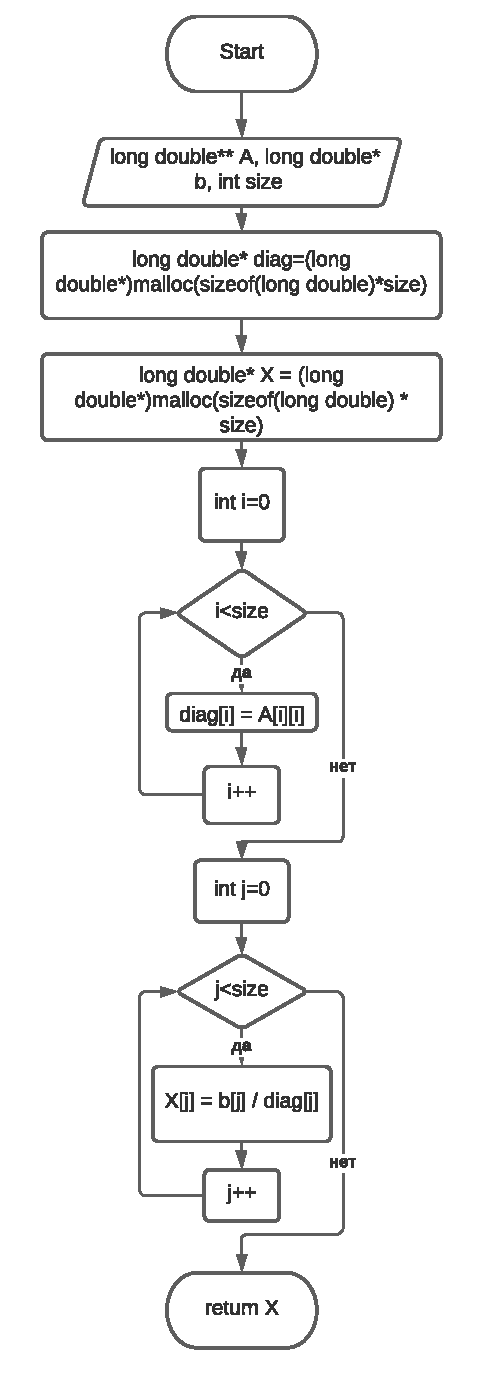
\includegraphics[scale=0.5]{block5.pdf}

double dTranFunc(double x)

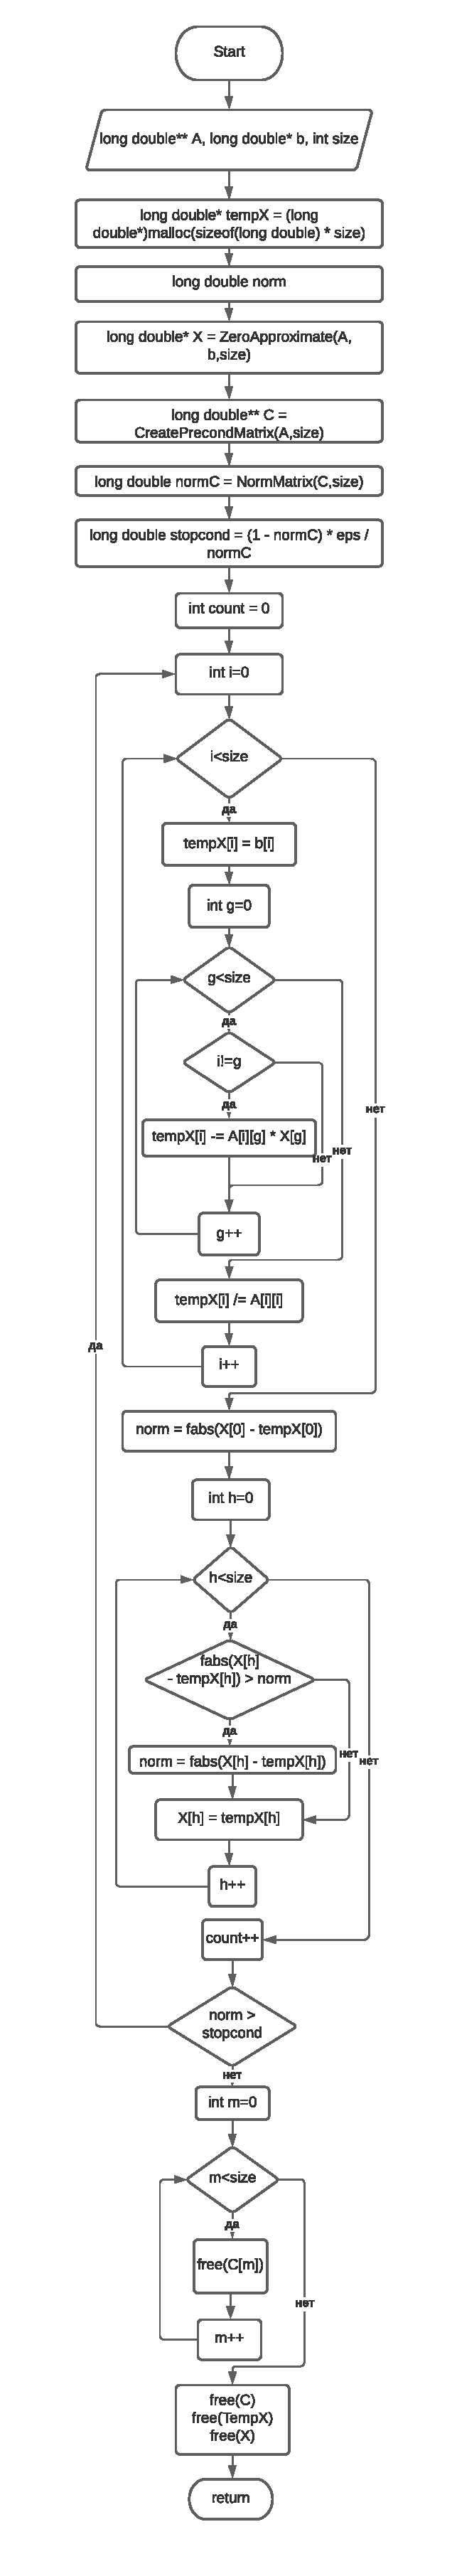
\includegraphics[scale=0.5]{block6.pdf}

void BisectionMethod(double(*func)(double), double left, double right, char const* filename)

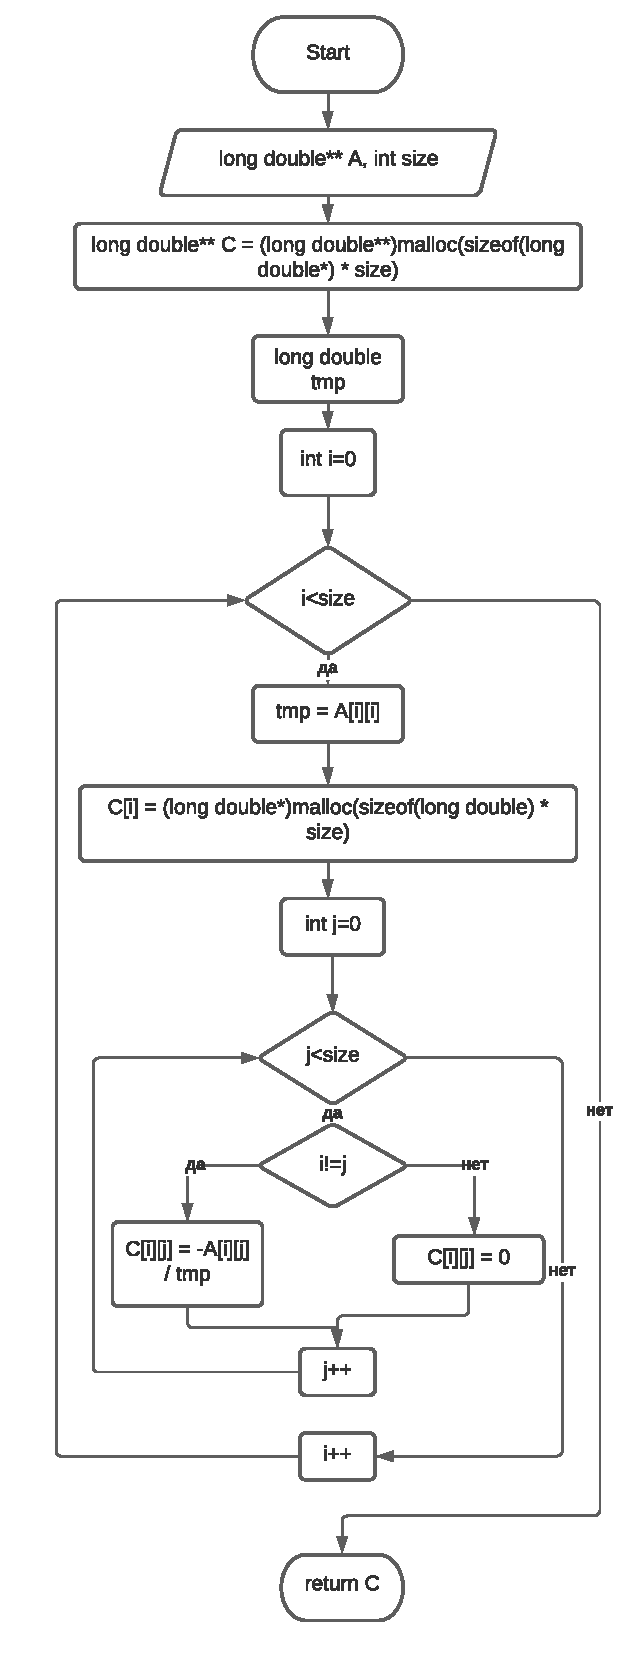
\includegraphics[scale=0.5]{block3.pdf}


void SecantMethod(double(*func)(double), double right, char const* filename, double(*dfunc)(double))

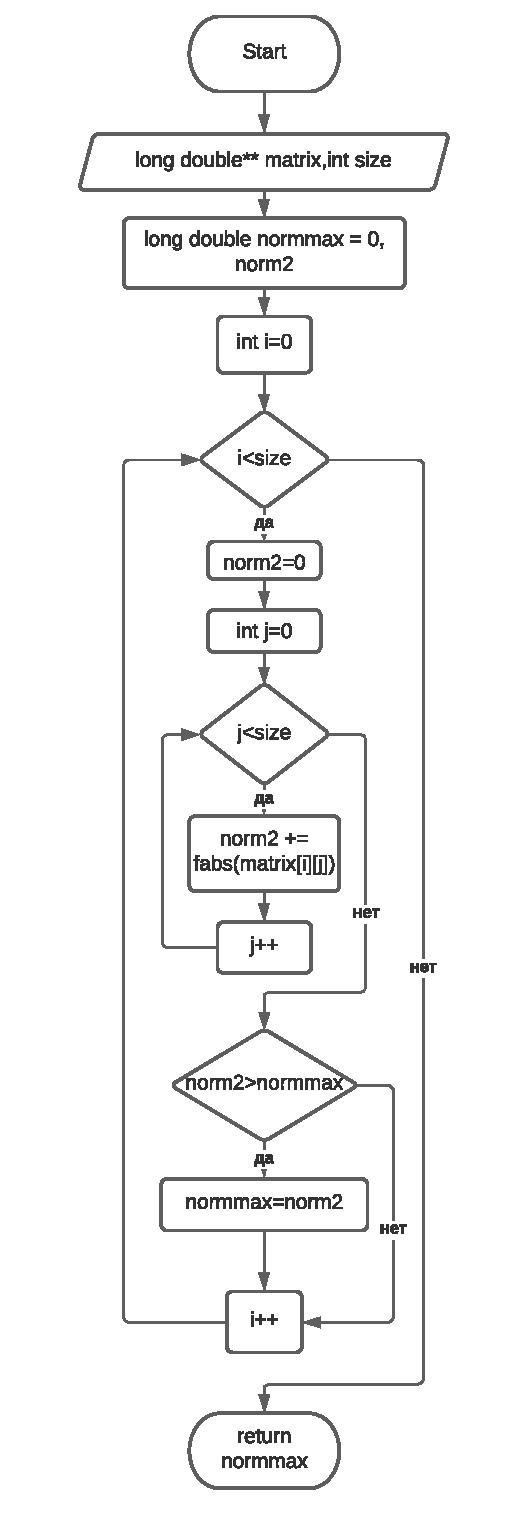
\includegraphics[scale=0.5]{block4.pdf}


\section{Численный анализ решения задачи}

\includegraphics[scale=0.75]{5.pdf}

На данном графике представлена зависимость количества итераций от заданной точности. Из графика можно сделать вывод, что чем меньше заданная точность, тем большее количество итераций необходимо для нахождения корня с заданной точностью (зависиимость стремится к линейной в логарифмическом масштабе). Также для поиска корня методом половинного деления требуется гораздо большее количество итераций, чем методом секущих, что особенно что хорошо отслеживается на маленьких значениях заданной точности. 

\includegraphics[scale=0.75]{6.pdf}

На данном графике представлена зависимость количества итераций от начального приближения. Из данного графика, как из предыдущего можно сделать вывод, что для поиска корня методом половинного деления требуется гораздо большее количество итераций, чем методом секущих. В случае с методом половинного деления при увеличении начального приближения для нахождения корня с заданной точнотью требуется большее количество итераций.Также можно сделать вывод, что процесс нахождения корня алгебраической функции более трудозатратный, нежели для трансцендентой функции.

\includegraphics[scale=0.75]{7.pdf}

На данном графике представлена зависимость абсолютной погрешности вычислений от количества итераций. Из данного графика можно сделать вывод, что метод секущих сходится быстрее,чем метод половинного деления, что становится особенно заметно при увеличении количества итераций. Метод секущих обладает сверхлинейной скоростью сходимости, а метод половинного деления скоростью, меньшую линейной

\includegraphics[scale=0.75]{8.pdf}

На данном графике представлена зависимость абсолютной погрешности вычислений от заданной точности. Из данного графика можно сделать вывод, что с увеличением точности погрешность уменьшается для обоих методов. 

\includegraphics[scale=0.75]{9.pdf}

На данном графике представлена графическая интерпретация метода секущих на примере алгебраической функции. Из графика видно, что каждое следующее приближение есть точка пересения прямой, проходящей через две точки на графике функции (данные точки являются значениями функций в точках двух предыдущих приближений), с осью абсцисс. 

\section{Краткие выводы}

Была решена задача нахождения корней алгебраического и трансцендентного уравнений с заданной точностью с использованием метода половинного деления и метода секущих.

Были выявлены зависимости количества итераций от заданной точности и начального приближения, а также зависимость погрешности от количества итераций (сходимость) и заданной точности.

Метод секущих является более быстрым и эффективным при одинаковых начальных условиях, чем метод половинного деления.


\end{document}
